\documentclass[paper=a4, fontsize=11pt]{article} % A4 paper and 11pt font size
\usepackage{amsmath,amsfonts,amsthm} % Math packages
\usepackage{fancyhdr} % Custom headers and footers
\pagestyle{fancyplain} % Makes all pages in the document conform to the custom headers and footers
\fancyhead{} % No page header - if you want one, create it in the same way as the footers below
\fancyfoot[L]{} % Empty left footer
\fancyfoot[C]{\thepage} % Empty center footer
\fancyfoot[R]{} % Page numbering for right footer
\renewcommand{\headrulewidth}{0pt} % Remove header underlines
\renewcommand{\footrulewidth}{0pt} % Remove footer underlines
\usepackage{graphicx}
\usepackage{indentfirst}
\usepackage[table]{xcolor}
\usepackage{booktabs}
\usepackage{tabularx}
\usepackage{amssymb,amsmath}

\newcommand{\ra}[1]{\renewcommand{\arraystretch}{#1}}
\setlength\parindent{20pt} % Removes all indentation from paragraphs - comment this line for an assignment with lots of text
\usepackage{amssymb}
% Margins
\topmargin=-0.45in
\evensidemargin=0.0in
\oddsidemargin=-0.5in
\hoffset=1.0in
\textwidth=5.5in
\textheight=9.0in
\headsep=0.25in

%----------------------------------------------------------------------------------------
%	TITLE SECTION
%----------------------------------------------------------------------------------------

\newcommand{\horrule}[1]{\rule{\linewidth}{#1}} % Create horizontal rule command with 1 argument of height

\title{	
\normalfont \normalsize 
\textsc{Norwegian University of Science and Technology} \\ [25pt] % Your university, school and/or department name(s)
\horrule{0.5pt} \\[0.4cm] % Thin top horizontal rule
\huge Particle Swarm Optimization\\ % The assignment title
\horrule{2pt} \\[0.5cm] % Thick bottom horizontal rule
}

\author{Jan Bednarik\\Tomas Dohnalek} % Your name

\date{\normalsize\today} % Today's date or a custom date

\begin{document}

\maketitle % Print the title

\section{Introduction}
This report describes the implementation of the Particle Swarm Optimization algorithm which can be utilized to solve various types of problems. In this case two standard problems will be solved using swarm intelligence -- Circle problems for both one and two dimensions and Knapsack problem.

The core part of the report is divided into four sections reflecting the single tasks of the assignment Particle Swarm Optimization introduced in course IT3105 - Artificial Intelligence Programming.
\section{Background}
The success rate of the standard Particle Swarm Optimization algorithm is mainly influenced by its parameters -- number of particles used, local attraction coefficient, global attraction coefficient to list the most important. Therefore it is crucial to choose the "right" values which would result in higher success rate. In the next paragraphs it will be explained why and which parameters were chosen for this project.

\subsection{Parameters}

\paragraph{Number of particles} Number of particles $N$ was chosen using following equation:

\begin{equation}
N = 10 + 2 \cdot \sqrt{D},
\end{equation}

where $D$ is dimension of the search space.

\paragraph{Local and global attraction coefficient}
It was empirically found that values close to $2.0$ give the best results. Given the limitations given by the assignment the value $1.999$ was chosen for both local and global attraction.

\subsection{Fitness function}
The core of the Particle Swarm Optimization is the fitness function. In most cases the objective of the algorithm is to minimize this function (while given the duality theorem it is also possible to maximize it in order to approximate the solution). It is relatively straightforward to solve the Circle problem as the search space has no local minimum (only one global).

The Knapsack problem search space is however significantly more complex tricky and what is more it is not convex. Thus the particles might reach the "forbidden" positions and the fitness function must reflect this. This specific implementation uses the approach of so called "death penalty". This means the particle reaching the unwanted area receives the fitness function value of +INFINITY. 

Thank to this approach the particles are able to discover very soon they should return to one of the allowed positions. The drawback of this approach is however the fact the particles might get stuck in local minimum.
\section{The circle problem}

This task is devoted to solving the Circle problem in the both one and two dimensional 
search spaces. The main objective was to obtain the fitness function value smaller than $0.001$.

The table \ref{tab:circle_1D_2D} shows the number of steps needed to achieve this goal in 10 different (independent) runs of both 1D and 2D circle problem. It can be noted that in most cases the 2D circle problem requires significantly more steps to be solved.

\begin{table*}[htb]
	\begin{center}
	\caption{Circle problem 1D and 2D -- 10 runs.}
	\label{tab:circle_1D_2D}
	\def\arraystretch{1.3}
		\begin{tabular}{ c c c }
		\toprule[0.5mm]
		& \multicolumn{2}{ c }{\textbf{Steps}} \\
		\textbf{\#} & \textbf{1D} & \textbf{2D}\\
		\midrule
				1  & 17 & 72 \\
				2  & 7 & 67 \\
				3  & 6 & 59 \\
				4  & 30 & 78 \\
				5  & 25 & 35 \\
				6  & 18 & 59 \\
				7  & 30 & 79 \\
				8  & 42 & 69 \\
				9  & 14 & 74 \\
				10 & 26 & 58 \\
		\bottomrule[0.5mm]
		\end{tabular}
	\end{center}
\end{table*}
\section{The circle problem with the nearest neighbour topology support}
In this task the circle problem is solved using the nearest neighbour topology. This means that the particles no longer represent fully connected topology but each particle rather considers only its specific surrounding.

Figure \ref{fig:2Dcircle_nntopology} shows the results for both 1D and 2D Circle problem with nearest neighbour topology support. In this case the particles only communicate their best global position to three nearest particles.

Figure \ref{fig:2Dcircle_nntopology_inertia} shows the results for both 1D and 2D Circle problem with nearest neighbour topology suppport. It also adds the support for the weighed inertia that influences the value of each particle's velocity. In this case the inertia gradually decreases from value $1.0$ to value $0.4$.

\begin{figure}[!h]
	\centering
		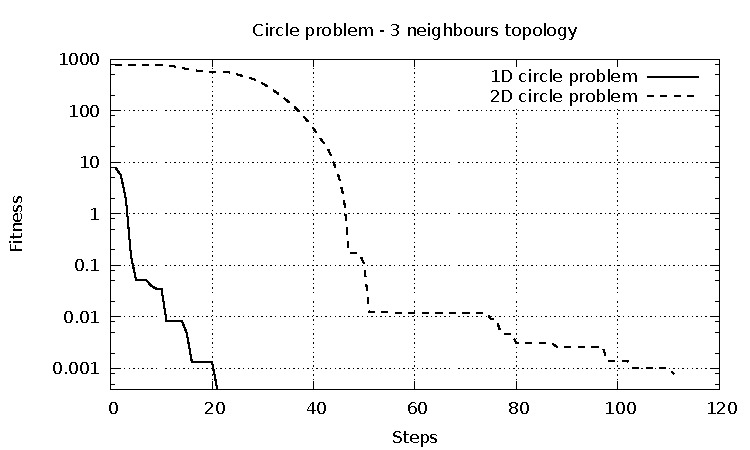
\includegraphics[width=15cm]{img/2a.pdf}
	\caption{2D circle problem with nearest neighbour topology (3 neighbours).}
	\label{fig:2Dcircle_nntopology}
\end{figure}

\begin{figure}[!h]
	\centering
		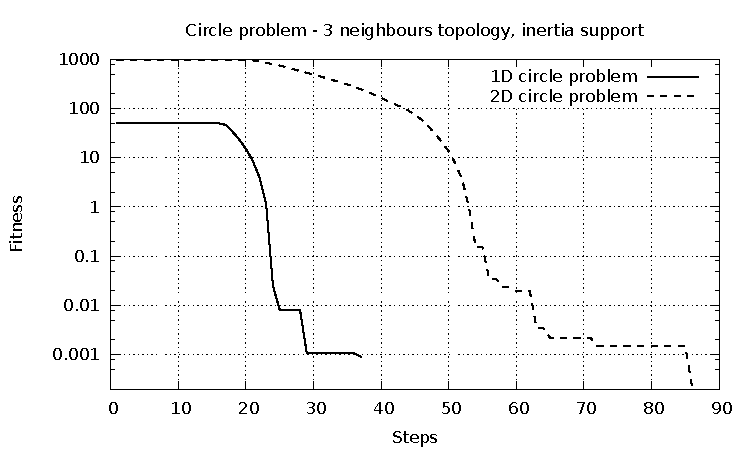
\includegraphics[width=15cm]{img/2b.pdf}
	\caption{2D circle problem with nearest neighbour topology (3 neighbours) and inertia support.}
	\label{fig:2Dcircle_nntopology_inertia}
\end{figure}
\section{0-1 knapsack problem}
This task describes the utilization of Particle Swarm Optimization algorithm utilized for solving so called Knapsack problem. In this task the amount of packages put inside the knapsack is only limited by the knapsack's weight limit.

It should be mentioned how the fitness function is represented. This specific implementation's aim is to minimize the value of fitness function which is expressed as the subtraction of the total value of all packages and the total value of packages present in the knapsack.

Figure \ref{fig:knaspack} shows the results of Particle Swarm Optimization algorithm used to solve the Knapsack problem with different values chosen for both local and global attraction coefficient. It can be seen that the algorithm gives the best result when both local and global attraction coefficients are set to the same value ($1.999$). If there is put focus either on local or global attraction the results are somewhat the same but worse as compared with the first case.

\begin{figure}[!h]
	\centering
		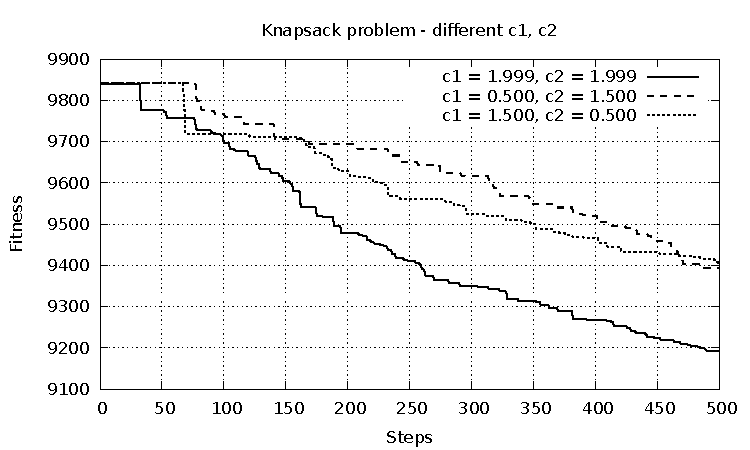
\includegraphics[width=15cm]{img/3b.pdf}
	\caption{Knapsack problem solution with different values for global and local attraction. The best result (full line) gained the fitness function value of 9191, while filling the knapsack up to 992.87 kg with total value of 722.4. The second best result (dashed line) gained the fitness function value of 9394, while filling the knapsack up to 997.56 kg with total value of 518.9. The worst result (dotted line) gained the fitness function value of 9406, while filling the knapsack up to 979.75 kg with total value of 506.9.}
	\label{fig:knaspack}
\end{figure}

Figure \ref{fig:knaspack} shows the results of Particle Swarm Optimization algorithm used to solve the Knapsack problem with different values chosen for both local and global attraction coefficient and with inertia support. It can be seen that no matter how many steps the result of the fitness function never changes. The reason might be the fact that due to the decreasing inertia and thus the decreasing velocity the particles are not able to search the wide are in search space and rather tend to return to their own best positions found.

\begin{figure}[!h]
	\centering
		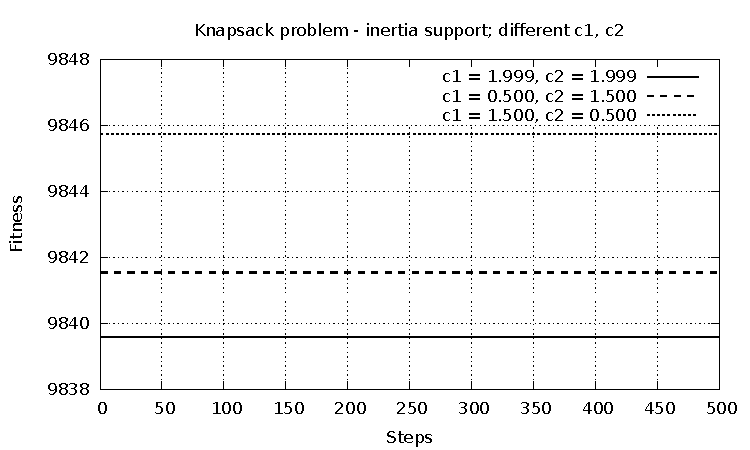
\includegraphics[width=15cm]{img/3c.pdf}
	\caption{Knapsack problem solution with different values for global and local attraction and support for inertia. Knapsack problem solution with different values for global and local attraction. The best result (full line) gained the fitness function value of 9840, while filling the knapsack up to 514.76 kg with total value of 73.9. The second best result (dashed line) gained the fitness function value of 9841, while filling the knapsack up to 578.9 kg with total value of 72.0. The worst result (dotted line) gained the fitness function value of 9846, while filling the knapsack up to 585.47 kg with total value of 67.76.}
	\label{fig:knaspack_inertia}
\end{figure}
\section{0-1 knapsack problem with volume extension}


\section{Summary}
The aim of this project was to utilize the Particle Swarm Optimization algorithm to solve the two well known standard problems called Circle problem and Knapsack problem. It was discovered the results are mainly influenced by the setting of local and global attraction coefficients and also by the utilization of the weighed inertia influencing the particles' velocity.

%-----------------------------------------------
\begin{flushleft}
%\bibliography{literatura} % viz. literatura.bib..
%\bibliographystyle{czplain}
\end{flushleft}
\end{document}
